\documentclass[11pt,a4paper]{article}

% ---------------------------------------------------------------- layout and fonts
\usepackage[T1]{fontenc}
\usepackage[utf8]{inputenc}
\usepackage{newtxtext,newtxmath}
\usepackage{sourcesanspro}
\renewcommand{\familydefault}{\rmdefault}
\usepackage[margin=2.5cm,top=2.4cm,bottom=2.6cm]{geometry}
\usepackage{microtype}
\usepackage{xcolor}
\usepackage{graphicx}
\usepackage{booktabs}
\usepackage{tabularx}
\usepackage{enumitem}
\usepackage[font=small,labelfont={sf,bf},labelsep=period]{caption}
\usepackage{titlesec}
\usepackage{fancyhdr}
\usepackage{amsmath}
\usepackage{float}
\usepackage{tikz}
\usetikzlibrary{arrows.meta,positioning}
\usepackage[round,authoryear]{natbib}
\usepackage[hidelinks]{hyperref}

\definecolor{accent}{RGB}{31,58,96}
\definecolor{muted}{RGB}{105,105,105}
\hypersetup{colorlinks=true,linkcolor=accent,urlcolor=accent,citecolor=accent,
  pdftitle={An LLM Tone Score for FOMC Statements and the 2-Year Yield},pdfauthor={Hadrien Tramoni}}

\newcommand{\sfb}[1]{{\sffamily\bfseries #1}}
\titleformat{\section}{\sffamily\bfseries\large\color{accent}}{\thesection}{0.7em}{}
\titleformat{\subsection}{\sffamily\bfseries\normalsize\color{accent}}{\thesubsection}{0.6em}{}
\titlespacing*{\section}{0pt}{1.15em}{0.45em}
\titlespacing*{\subsection}{0pt}{0.8em}{0.25em}

\setlist{itemsep=0.15em,topsep=0.35em,leftmargin=1.4em}
\setlength{\parskip}{0.5em}
\setlength{\parindent}{0pt}
\renewcommand{\arraystretch}{1.12}

\pagestyle{fancy}
\fancyhf{}
\renewcommand{\headrulewidth}{0pt}
\fancyhead[L]{\sffamily\footnotesize\color{muted}An LLM Tone Score for FOMC Statements and the 2-Year Yield}
\fancyhead[R]{\sffamily\footnotesize\color{muted}H.~Tramoni}
\fancyfoot[C]{\sffamily\footnotesize\color{muted}\thepage}
\fancypagestyle{first}{\fancyhf{}\fancyfoot[C]{\sffamily\footnotesize\color{muted}\thepage}}

\newcommand{\doi}[1]{\href{https://doi.org/#1}{doi:#1}}
\newcommand{\bp}{\,bp}
\newcommand{\sd}{\,SD}

\begin{document}
\thispagestyle{first}

% ---------------------------------------------------------------- title block
\begin{flushleft}
{\sffamily\small\color{muted} Working paper \quad$\cdot$\quad November 2026}\\[0.6em]
{\sffamily\bfseries\LARGE\color{accent} An LLM Tone Score for FOMC Statements and the 2-Year Yield}\\[0.7em]
{\normalsize Hadrien Tramoni}\\[0.2em]
{\small\color{muted} Code, data pipeline and full protocol:
\href{https://github.com/HadrienT/text-signals}{github.com/HadrienT/text-signals}}
\end{flushleft}

\vspace{0.4em}
\noindent\colorbox{accent!6}{\parbox{\dimexpr\textwidth-2\fboxsep}{\small
\sfb{Abstract.}
A local 14\,B open-weight model (Phi-4) reads each FOMC statement from 1994 to 2026 into a
structured extraction with verbatim evidence. Its aggregate tone score explains the 2-year
Treasury yield's move in the 30 minutes around the release, beyond the rate surprise and two
standard text baselines. A one-standard-deviation more hawkish statement comes with a
$+1.03$\bp{} move (HAC $p = 0.004$, $n = 243$), under a specification fixed before any score
met market data. The effect survives every pre-specified robustness check and a permutation
placebo, and adds 2.1\% out-of-sample $R^2$ over the baseline. It is also narrow: it does not
reach the daily close, it is weak on press conference days, and its out-of-sample gain was
earned before 2009 and in 2022. Because the model has read the history of almost every
statement, look-ahead bias is tested from several angles. The decisive one rewrites each
statement's forward guidance: the score follows the text every time, as much for statements
the model may remember as for those it cannot. A frontier model gives the same signal with
cleaner extraction. A retrieval agent built on the same corpus answers most questions
correctly with verbatim citations, but it also shows how such citations can mislead.}}

\vspace{0.6em}

% ================================================================
\section{Question and design}

When the Federal Open Market Committee releases a statement, the rate decision is usually
priced in. What moves bonds is what the text implies about the future path of policy
\citep{gss2005}. This paper asks two questions. Can an LLM reading only
the text measure that stance well enough to explain the market's reaction, beyond the decision
and beyond dictionary and encoder baselines? And how much of the result survives once
look-ahead bias is addressed?

\begin{figure}[H]
\centering
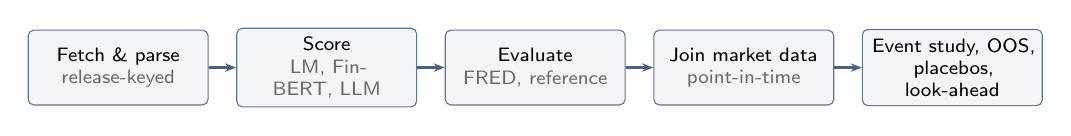
\begin{tikzpicture}[
  box/.style={draw=accent!70,fill=accent!5,rounded corners=2pt,font=\sffamily\scriptsize,
    align=center,minimum height=0.95cm,text width=2.05cm},
  arr/.style={-{Stealth[length=4pt]},accent!80,thick}]
\node[box] (f) {Fetch \& parse\\{\color{muted}release-keyed}};
\node[box,right=0.35cm of f] (s) {Score\\{\color{muted}LM, FinBERT, LLM}};
\node[box,right=0.35cm of s] (e) {Evaluate\\{\color{muted}FRED, reference}};
\node[box,right=0.35cm of e] (j) {Join market data\\{\color{muted}point-in-time}};
\node[box,right=0.35cm of j] (t) {Event study, OOS,\\placebos, look-ahead};
\draw[arr] (f)--(s); \draw[arr] (s)--(e); \draw[arr] (e)--(j); \draw[arr] (j)--(t);
\end{tikzpicture}
\caption{The pipeline. Every document is keyed by its release timestamp, and every LLM output is
cached with its model, weights, prompt and schema versions.}
\end{figure}

\sfb{Event and outcome.} There is one observation per statement: the change in the 2-year
yield in the 30-minute window around the release, from the San Francisco Fed's event-study
database \citep[USMPD;][]{acosta2025}. The window
isolates the statement from the press conference and same-day news; the daily change is kept
as a robustness outcome. Release dates were checked against four sources, and two calendar
errors and four misdated minutes in the intraday database were corrected.

\sfb{Model.} The model is estimated by OLS,
\[
  \Delta y_i = \alpha + \beta\,\mathrm{tone}_i + \gamma\,\mathrm{MP1}_i
  + \delta'\,\mathrm{baselines}_i + \varepsilon_i ,
\]
where MP1 is the futures-based surprise in the rate decision \citep{kuttner2001}, defined in
Appendix~\ref{app:mp1}. The baselines are the \citet{lm2011} net negative share and the mean
$P(\text{neg}) - P(\text{pos})$ of FinBERT \citep{araci2019}. Inference uses Newey--West
standard errors \citep{neweywest1994} with 4 lags, chosen a priori. There is one primary
test ($H_0\!: \beta = 0$), and the 14 secondary tests are corrected together by Holm. Power was
computed before scoring: about 0.92\bp{} per SD is detectable with 80\% power. The sample has
250 statements; 243 enter the primary test.

% ================================================================
\section{Measuring tone}

The model fills a typed schema: five stance fields on a common $-2$ (dovish) to $+2$ (hawkish)
scale (forward guidance, inflation, labour market, growth, balance sheet), the risk balance,
the decision with its size, and dissents. Every field carries a span copied verbatim from the
statement as evidence. The tone score is the equal-weight mean of the filled stance fields, so
no weight is fitted to the outcome.

There is no ground truth for the extraction. Hand labelling was stopped after five practice
statements, and a stronger model (Claude Opus 5.5) served as a blind \emph{reference reader}. Agreement
with it measures consistency, not correctness. Two checks need no reader: the decision and its
size against FRED, and whether each evidence span appears verbatim. On a fresh confirmation
sample, fixed in advance, Phi-4 gave 0 invalid outputs, a tone correlation of 0.86 with the
reference and a forward guidance $\kappa$ of 0.62. Rejected choices are reported too: a model
that inverted the sign of balance-sheet purchases ($\kappa = 0.07$), an evidence-by-sentence
schema that collapsed the forward guidance $\kappa$ (0.84 to 0.30), and a repair loop that
changed values. In the end, scores use the model's first answer only.

% ================================================================
\section{Results}

\subsection{Primary test}

\begin{table}[H]
\centering\small
\begin{tabular}{lrr}
\toprule
Regressor & $\beta$ per SD (bp) & HAC $p$ \\
\midrule
LLM tone (Phi-4)                & $\mathbf{+1.03}$ & $\mathbf{0.004}$ \\
MP1 (rate surprise)             & $+2.11$ & 0.002 \\
Loughran--McDonald net negative & $-0.39$ & 0.28 \\
FinBERT net negative            & $-0.00$ & 0.99 \\
\bottomrule
\end{tabular}
\caption{Primary test, 30-minute change in the 2-year yield, $n = 243$. $R^2$ rises from
0.198 to 0.221 when the LLM score is added; the baselines carry nothing once it is in.}
\end{table}

\begin{table}[H]
\centering\small
\begin{tabular}{lrr}
\toprule
Robustness check (all fixed in advance) & $\beta$ per SD (bp) & $p$ \\
\midrule
HC3 standard errors                                 & 1.03 & 0.014 \\
Moving-block bootstrap, 95\% interval               & 1.03 & [0.36, 1.77] \\
Without the 19 influential statements (Cook's 4/$T$) & 1.01 & 0.001 \\
Huber robust regression                             & 0.73 & 0.022 \\
\bottomrule
\end{tabular}
\caption{Robustness. Residuals are heteroskedastic and fat-tailed but not autocorrelated, and
collinearity is negligible (VIF $\le 1.63$).}
\end{table}

\subsection{Where the effect stops}

Five of the 14 secondary tests survive Holm. The ones that bound the result:
\begin{itemize}
\item \sfb{No effect on the daily close} ($-0.07$\bp{} per SD, $p = 0.91$). The tone moves
  yields inside the window. Nothing here shows the move lasts: it may be reversed or swamped
  later in the day, or the daily change may be too noisy.
\item \sfb{Much weaker on press conference days}: $+0.48$ ($n = 96$) against $+1.70$ on other
  days. When the Chair speaks 30 minutes later, markets seem to wait, and since 2019 that is
  every meeting.
\item The change in tone from the previous statement points the same way ($+0.85$) but does
  not survive correction (Holm $p = 0.079$).
\end{itemize}

\subsection{Out of sample and placebos}

The model is refitted every January on past statements only and forecasts that year, from
2000 to 2026. Adding the LLM score lowers the squared forecast error by \sfb{2.1\%} against
the baseline; the Clark--West test of equal accuracy rejects with one-sided $p = 0.003$
\citep{clarkwest2007}. The gain is not steady (Figure~\ref{fig:oos}).

\begin{figure}[H]
\centering
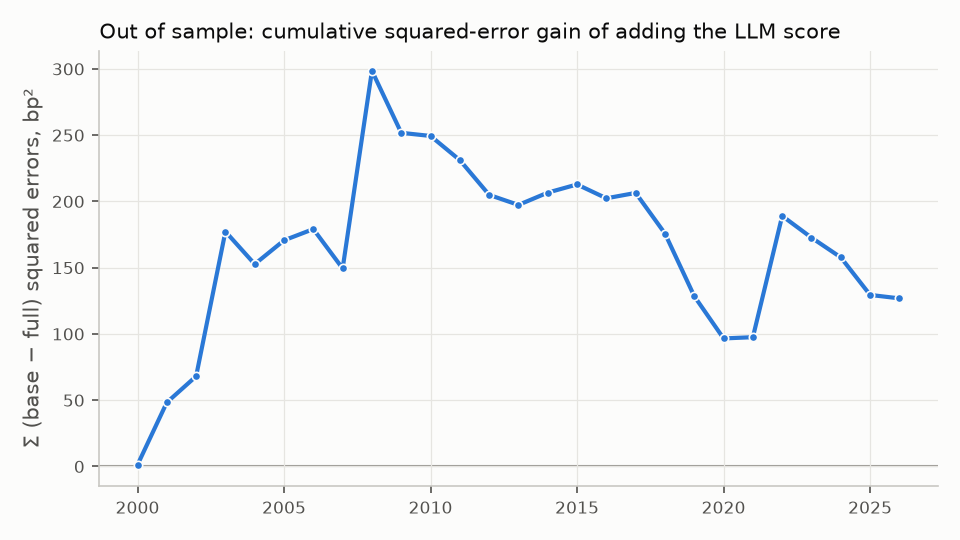
\includegraphics[width=0.6\textwidth]{../docs/case-studies/figures/fomc_oos_cumulative_gain.png}
\caption{Cumulative out-of-sample squared-error gain of adding the LLM score. It is earned in
2000--2008 and in 2022, and lost in most other years; on recent years alone, the score would
not have helped a forecaster.}
\label{fig:oos}
\end{figure}

Shuffling the score across statements (9,999 permutations) leaves $t$-statistics centred on
zero, and the observed $t$ of 2.85 lies beyond 99.5\% of them. The previous statement's score
explains nothing on its own. One placebo expectation failed. Placed next to the current score,
the previous one is significantly negative ($-1.04$, $p = 0.034$), as if the market priced the
new tone net of the tone already known. That reading was formed after the result and is not
tested.

% ================================================================
\section{Look-ahead bias}

Phi-4's training data end in June 2024, so it has read the history of 230 of the 250
statements. A model that knows how markets took a statement could let that shade its reading.

\begin{table}[H]
\centering\small
\begin{tabularx}{\textwidth}{>{\raggedright\arraybackslash}p{3.3cm}X}
\toprule
Test & Result \\
\midrule
Cutoff split & $\beta = -0.44$ (se 1.38) on the 19 statements after the cutoff: not
  detectable; no power, stated in advance. \\
Regime-matched split & On press conference days before the cutoff, $\beta = +0.56$
  ($n = 77$): inconclusive by the pre-set rule. The regime halves the effect but does not
  remove it. \\
Anonymisation & With dates and names removed, scores correlate 0.96 with the originals;
  $\beta$ is 0.85 against 0.97. \\
Dating probe & The model dates anonymised statements: 81\% within one year, but it never
  places a statement after 2023. It knows the period. \\
Look-ahead-free reader & Models trained only on earlier text (ChronoGPT vintages, \citealp{he2025}) cannot read
  the statements ($r = 0.04$ against a 0.30 bar): no evidence either way. \\
\textbf{Counterfactual edits} & \textbf{On 38 statements, a hawkish rewrite of the guidance
  sentence beats the dovish one 100\% of the time, before and after the cutoff alike.}
  Statements the model may remember move slightly more ($+0.33$, 95\% interval $-0.07$ to
  $+0.68$). \\
\bottomrule
\end{tabularx}
\caption{Look-ahead tests. The edits were written and frozen before any edited text was read.}
\end{table}

Look-ahead needs two steps: the model knows the period, and that knowledge shades the score.
The probe shows the first. The counterfactual edits test the second directly and do not find
it. Two statements, one on each side of the cutoff, share the same guidance sentence and got
identical rewrites, and the model reads them identically. Statements whose text kept other
guidance sentences, which would pull the reading back as memory would, were flagged in advance,
and the result holds without them. Look-ahead is not excluded, since memory could still shade
borderline readings where text and memory agree, but nothing found indicates that it drives
the result.

% ================================================================
\section{Does a frontier model read better?}

As an exploratory second reader, specified before any reading, Claude Opus 5.5 scored all 250
statements. For economy it read them in batches rather than one per call as the local model
did, on anonymised texts shuffled across years to limit recognition.

\begin{table}[H]
\centering\small
\begin{tabular}{lccc}
\toprule
 & Phi-4, original & Phi-4, anonymised & Claude, anonymised \\
\midrule
Decision right (FRED)              & -- & 96\% & 96\% \\
Statements with non-verbatim evidence & -- & $\sim$33\% & \textbf{0\%} \\
$\beta$ per SD (bp), HAC $p$       & 0.97, 0.006 & 0.84, 0.012 & 0.90, 0.007 \\
Out-of-sample $R^2$ vs baseline    & 2.6\% & 1.3\% & 0.4\% \\
\bottomrule
\end{tabular}
\caption{Same 239 statements throughout. The two tone scores correlate at 0.89, and in a joint
regression neither adds to the other.}
\end{table}

The frontier model extracts more cleanly but finds no stronger signal. The tone of a statement
is coarse enough that a 14\,B local model captures what moves the 2-year yield. The comparison
also gives an indirect argument on look-ahead. Claude's training data cover all but three
statements, so if knowing what followed drove the scores, the model that knows most should fit
best, and it does not.

% ================================================================
\section{A retrieval agent, and how far its citations can be trusted}

A separate question is reliability: when an LLM answers a research question and cites its
sources, can the citations be trusted? A question-answering agent over the corpus (250
statements, 262 sets of minutes, 96 press conference transcripts; 26,354 passages) combines
BM25 and a dense encoder by reciprocal rank fusion, with an \texttt{as\_of} filter for the
point-in-time rule. Phi-4 answers from the top eight passages with verbatim quotes, or refuses,
and code checks every quote. Fifty questions with reference passages were written before any
answer, split into 10 for development and 40 for a single test run; ten were traps the agent
should refuse.

\begin{table}[H]
\centering\small
\begin{tabular}{lr}
\toprule
Test set, 40 questions & Result \\
\midrule
Retrieval recall@8 (fusion; BM25 0.50, encoder 0.53) & 0.59 \\
Answerable: right / partial / wrong / refused (of 32)   & 21 / 6 / 1 / 4 \\
Traps refused                                           & 6 of 8 \\
Citations verbatim (none invented)                      & 60 of 63 \\
\bottomrule
\end{tabular}
\caption{Indexing each passage with a header from its document's metadata, a change made on the
development questions, raised recall@8 from 0.25 to 0.59 on the test set.}
\end{table}

Three lessons apply to any such tool. \sfb{Retrieval is the bottleneck}: when the right passage
is retrieved, the answer is almost always right. \sfb{Citations are reliable word for word, but
not in time}: two answers quote exact text from the wrong meeting, attributing a June 2022
dissent to March 2022, and checking the quote alone would not catch it. \sfb{A point-in-time
filter is not enough}: asked ``as of'' 1 December 2015, before the first rate rise, the agent
gave the correct range, which appears in none of the retrieved passages. It answered from
memory, against its instructions: look-ahead in miniature.

% ================================================================
\section{Limitations}

\begin{itemize}
\item \sfb{Small sample, wide intervals.} With 243 events, the estimate is close to the minimum
  detectable effect.
\item \sfb{Narrow effect.} It is intraday only and weak when a press conference follows, which
  limits its relevance to today's FOMC.
\item \sfb{No ground truth} for the extraction; the hardest field, forward guidance, has a
  $\kappa$ of 0.6--0.7 out of sample.
\item The intraday data are taken from USMPD as published.
\item \sfb{Negative and failed results} are reported in the protocol: the daily outcome, the
  change in tone, a failed placebo expectation, a look-ahead-free reader too weak to use, an
  inconclusive regime test, rejected extraction variants and an imperfect trap question.
\item \sfb{Labelled post-hoc choices.} Choices made after seeing a result are labelled as such,
  and each was made on development data before a single test run.
\end{itemize}

% ================================================================
\section{Implications and next step}

For investment research, a local open-weight model gives an auditable, verbatim-sourced reading
of central bank text with a measurable link to rates. It costs nothing at the margin, and no
document leaves the machine; for this task, a frontier model buys auditability, not signal. The
link is real but narrow, so it is one input to a rates view, not a strategy. Look-ahead bias
needs experiments of its own. Here, cutoff splits had no power and anonymisation removed too
little, and editing the text was what separated reading from remembering.

The two halves of the work can be joined. The failed placebo suggests that markets respond to
tone \emph{relative to what was already known}. The retrieval agent can measure this directly.
With the \texttt{as\_of} filter set to the day before each release, it can retrieve the
previous statement, the latest minutes and the latest press conference, and ask the model what
the new statement changes, with evidence on both sides. That score is point-in-time by
construction. Because the idea came from a result already seen, it would have to be specified
and frozen before computing it, and reported as exploratory.

\vspace{0.4em}
\noindent{\small\color{muted}\sfb{Reproducibility.} Everything a result depends on lives in
the repository and is tested. Raw files are stored with URL, fetch time and sha256, and every
LLM output with model, weights, prompt and schema versions. \texttt{just results} recomputes
every number in this paper from the data and caches. The protocol records each decision with
its date and reason.}

% ================================================================
\section*{Data and software}
{\small
\begin{itemize}[leftmargin=1.2em]
\item FOMC statements, minutes and press conference transcripts: Board of Governors of the
  Federal Reserve System,
  \href{https://www.federalreserve.gov/monetarypolicy/fomccalendars.htm}{federalreserve.gov/monetarypolicy/fomccalendars.htm}.
\item Intraday yield changes and the MP1 surprise: U.S. Monetary Policy Event-Study Database,
  Federal Reserve Bank of San Francisco, \href{https://sffed.us/usmpd}{sffed.us/usmpd}.
\item Daily Treasury yields and the federal funds target: FRED, Federal Reserve Bank of St.\ Louis,
  \href{https://fred.stlouisfed.org/}{fred.stlouisfed.org}.
\item Loughran--McDonald master dictionary:
  \href{https://sraf.nd.edu/loughranmcdonald-master-dictionary/}{sraf.nd.edu/loughranmcdonald-master-dictionary}.
\item Phi-4, Q8\_0 GGUF weights:
  \href{https://huggingface.co/microsoft/phi-4-gguf}{huggingface.co/microsoft/phi-4-gguf}.
\item FinBERT: \href{https://huggingface.co/ProsusAI/finbert}{huggingface.co/ProsusAI/finbert}.
  Retrieval encoder bge-small-en-v1.5:
  \href{https://huggingface.co/BAAI/bge-small-en-v1.5}{huggingface.co/BAAI/bge-small-en-v1.5}.
  ChronoGPT vintages: \href{https://huggingface.co/manelalab}{huggingface.co/manelalab}.
\item Code, protocol and data pipeline:
  \href{https://github.com/HadrienT/text-signals}{github.com/HadrienT/text-signals}.
\end{itemize}}

{\small
\renewcommand{\refname}{References}
\setlength{\bibsep}{0.25em}
\begin{thebibliography}{99}
\bibitem[Acosta et~al.(2025)]{acosta2025}
Acosta, M., Ajello, A., Bauer, M., Loria, F. and Miranda-Agrippino, S. (2025).
Financial market effects of FOMC communication: Evidence from a new event-study database.
\emph{Federal Reserve Bank of San Francisco Working Paper} 2025-30. \doi{10.24148/wp2025-30}.

\bibitem[Araci(2019)]{araci2019}
Araci, D. (2019). FinBERT: Financial sentiment analysis with pre-trained language models.
\href{https://arxiv.org/abs/1908.10063}{arXiv:1908.10063}.

\bibitem[Clark and West(2007)]{clarkwest2007}
Clark, T.~E. and West, K.~D. (2007). Approximately normal tests for equal predictive accuracy
in nested models. \emph{Journal of Econometrics} 138(1), 291--311.
\doi{10.1016/j.jeconom.2006.05.023}.

\bibitem[G\"urkaynak et~al.(2005)]{gss2005}
G\"urkaynak, R., Sack, B. and Swanson, E. (2005). Do actions speak louder than words? The
response of asset prices to monetary policy actions and statements. \emph{International Journal
of Central Banking} 1(1), 55--93.
\href{https://www.ijcb.org/journal/v1n1/do-actions-speak-louder-words-response-asset-prices-monetary-policy-actions-and}{ijcb.org}.

\bibitem[He et~al.(2025)]{he2025}
He, S., Lv, L., Manela, A. and Wu, J. (2025). Chronologically consistent large language models.
\href{https://arxiv.org/abs/2502.21206}{arXiv:2502.21206}.

\bibitem[Kuttner(2001)]{kuttner2001}
Kuttner, K.~N. (2001). Monetary policy surprises and interest rates: Evidence from the Fed funds
futures market. \emph{Journal of Monetary Economics} 47(3), 523--544.
\doi{10.1016/S0304-3932(01)00055-1}.

\bibitem[Loughran and McDonald(2011)]{lm2011}
Loughran, T. and McDonald, B. (2011). When is a liability not a liability? Textual analysis,
dictionaries, and 10-Ks. \emph{Journal of Finance} 66(1), 35--65.
\doi{10.1111/j.1540-6261.2010.01625.x}.

\bibitem[Nakamura and Steinsson(2018)]{ns2018}
Nakamura, E. and Steinsson, J. (2018). High-frequency identification of monetary
non-neutrality: The information effect. \emph{Quarterly Journal of Economics} 133(3),
1283--1330. \doi{10.1093/qje/qjy004}.

\bibitem[Newey and West(1994)]{neweywest1994}
Newey, W.~K. and West, K.~D. (1994). Automatic lag selection in covariance matrix estimation.
\emph{Review of Economic Studies} 61(4), 631--653. \doi{10.2307/2297912}.
\end{thebibliography}}

% ================================================================
\appendix
\section{The MP1 surprise}
\label{app:mp1}

MP1 measures how much the rate decision itself surprised the market, using fed funds futures
\citep{kuttner2001}. A fed funds futures contract for a given month settles on the
\emph{average} effective federal funds rate over that month, and its implied rate is
$100 - \text{price}$. Its change in a narrow window around a release therefore reveals how the
market's expectation for the month moved when the decision became known.

Let $\Delta f^{1}$ be the change in the implied rate of the current-month contract between 10
minutes before and 20 minutes after the release, $D$ the number of days in the month and $d$
the day of the meeting. A change in the rate decided on day $d$ only affects the remaining
$D - d$ days of the monthly average, so the surprise in the rate itself is
\[
  \mathrm{MP1} = \frac{D}{D - d}\,\Delta f^{1} .
\]
When the meeting falls in the last seven days of the month, the scaling factor becomes large
and noisy, and the change in the next month's contract, $\Delta f^{2}$, is used instead.

\sfb{Example.} For a meeting on the 16th of a 30-day month, a 5\bp{} rise in the current-month
implied rate means that the decided rate was $5 \times 30/14 \approx 10.7$\bp{} above what the
market expected.

\sfb{Source and checks.} The values come from the USMPD \citep{acosta2025}. We recomputed MP1 from
the database's futures changes and matched it on all 280 statements. In the primary sample, its
standard deviation is 6.9\bp{}.

\sfb{Why MP1 and not a broader surprise.} The database also provides a surprise built from
futures over about a year \citep{ns2018}. That measure includes the market's reaction to forward
guidance, the very content the text score is meant to capture, so using it as a control would
absorb the effect under study. MP1 removes only the surprise in the current decision.

\end{document}
